\section{Generative Artificial Intelligence}

\begin{definition}[\textit{Generative Artificial Intelligence}]
    Generative AI is a branch of artificial intelligence focused on creating systems that can generate new data samples, which closely resemble those in the training dataset.
\end{definition}
\noindent Unlike discriminative models, which are designed to classify input data into predefined categories or make specific predictions, generative models aim to learn the underlying structure of the data and generate new instances that reflect the distribution of that data.
In essence, generative AI seeks to replicate the creativity and generative abilities of humans by learning from examples and producing new content with similar characteristics.
These models are trained on large datasets and can generate realistic data across a variety of domains.

\paragraph*{Applications}
Generative AI has a wide range of applications across different domains, including:
\begin{itemize}
    \item \textit{Image generation and editing}: Generative Adversarial Networks are commonly used to generate realistic images. 
        They are also effective for image-to-image translation tasks, such as style transfer and colorization.
    \item \textit{Text Generation and summarization}: language models can generate coherent, contextually relevant text. 
    \item \textit{Content creation and augmentation}: generative AI can be used to create entirely new forms of content, including music, videos, and artwork. 
        Additionally, these models can enhance existing content by generating variations or filling in missing parts.
    \item \textit{Data synthesis and simulation}: generative models can create synthetic data that closely resembles real-world data, making them useful for data augmentation, training machine learning models, and simulating realistic scenarios. 
\end{itemize}

\begin{definition}[\textit{Large Language Models}]
    A Large Language Model is a type of artificial intelligence designed to understand and generate human-like text based on the input it receives.
\end{definition}
\noindent These models are trained on vast amounts of text data, typically sourced from the internet or other extensive corpora, in order to learn the complex patterns and structures of human language.

Large language models are typically built using deep learning architectures, often based on transformer architectures. 
These models consist of multiple layers of neural networks that process input text in a hierarchical manner, capturing both local and global dependencies in the text. 
The result is a model capable of producing highly coherent and contextually relevant text.

Once trained, LLMs are capable of performing a wide variety of natural language processing tasks, including text generation, text completion, translation, summarization, and question answering. 
The ability of LLMs to generate text that is contextually appropriate and fluent has made them widely used in many applications, including virtual assistants, content creation, and more.

\paragraph*{Prompt engineering}
\begin{definition}[\textit{Prompt engineering}]
    Prompt engineering is the practice of designing and crafting prompts or inputs that are used to interact with language models or AI systems in order to achieve specific, desired outputs. 
\end{definition}
\noindent The goal is to optimize how questions or requests are framed to ensure the AI generates accurate, useful, and relevant responses.
Key tips for effective prompting include being clear and specific, providing relevant context, asking open-ended questions, using important keywords, avoiding ambiguity, engaging in conversation, offering feedback, and experimenting with different approaches.

\subsection{Multimodal generative AI}
Multimodal generative AI refers to systems that can create content across multiple modalities. 
These advanced AI systems use machine learning techniques to process and generate content from various data types.

Unlike traditional generative models that focus on a single modality, multimodal models can handle multiple data types at once, enabling more expressive and comprehensive content generation.
These models understand the relationships between different forms of data.
This cross-modal understanding results in more contextually relevant and dynamic content.

\paragraph*{Training}
Training multimodal AI models requires large, diverse datasets that include paired examples of different data types
These datasets help the model learn the correlations and connections between various modalities, enhancing its ability to generate accurate and coherent content across different forms of media.

\subsection{Ethic}
Generative AI raises several ethical concerns that need careful consideration. 

\renewcommand{\arraystretch}{1.5}
\begin{table}[!ht]
    \centering
    \begin{tabular}{|l|p{10cm}|}
    \hline
    \textbf{Ethical concern} & \textbf{Description} \\
    \hline
    Misinformation & Generative AI can create convincing fake content, leading to misinformation and manipulation \\
    \hline
    Privacy Concerns & Models may inadvertently reproduce sensitive information, risking privacy violations \\
    \hline
    Bias and Fairness & AI models can perpetuate biases, leading to unfair or discriminatory outcomes \\
    \hline
    Intellectual Property & AI-generated content raises issues about ownership and copyright infringement \\
    \hline
    Security Risks & AI can be misused for malicious activities, such as phishing or creating deepfakes \\
    \hline
    Identity Theft & Generative AI may be used for identity theft, fraud, and other criminal activities \\
    \hline
    Regulatory Challenges & Current laws may not fully address the complexities of generative AI technology \\
    \hline
    Creative Industries & AI could disrupt creative fields, leading to job displacement and economic challenges \\
    \hline
    \end{tabular}
    \caption{Ethical concerns in generative AI}
\end{table}
\renewcommand{\arraystretch}{1}

\subsection{Enterprise applications}
\begin{definition}[\textit{Retrieval Augmented Generation}]
    Retrieval Augmented Generation is a technique in natural language processing that combines retrieval-based methods with generative models to improve the quality and relevance of generated text.
\end{definition}
\noindent In RAG, a retriever component searches a large database or text corpus to find information relevant to the input query or context.
This information is then used to enhance the generative model's process producing more accurate, coherent, and contextually relevant responses. 
With RAG, company data can be used to enrich prompts. 

\paragraph*{Architectures}
\noindent In the enterprise architectures with generative AI, we have the following components:
\begin{itemize}
    \item \textit{Vectorial database layer}: a storage layer that organizes data in a format easily understood by a large language model.
    \item \textit{Feedback}: a system to collect feedback and contextual information, allowing for continuous improvement and evolution of the model.
    \item \textit{RAG agent}: the core component of the system responsible for managing inputs and outputs.
    \item \textit{Guard eail}: a safeguard to prevent model leakage or malicious attacks, ensuring the quality and security of outputs. 
        Limiting the LLM's ability can result in performance degradation and increased latency as all inputs and outputs must be checked.
    \item \textit{LLM gateway and catalog}: this component is responsible for routing prompts to the most suitable LLM for processing.
\end{itemize}

\begin{figure}[H]
    \centering
    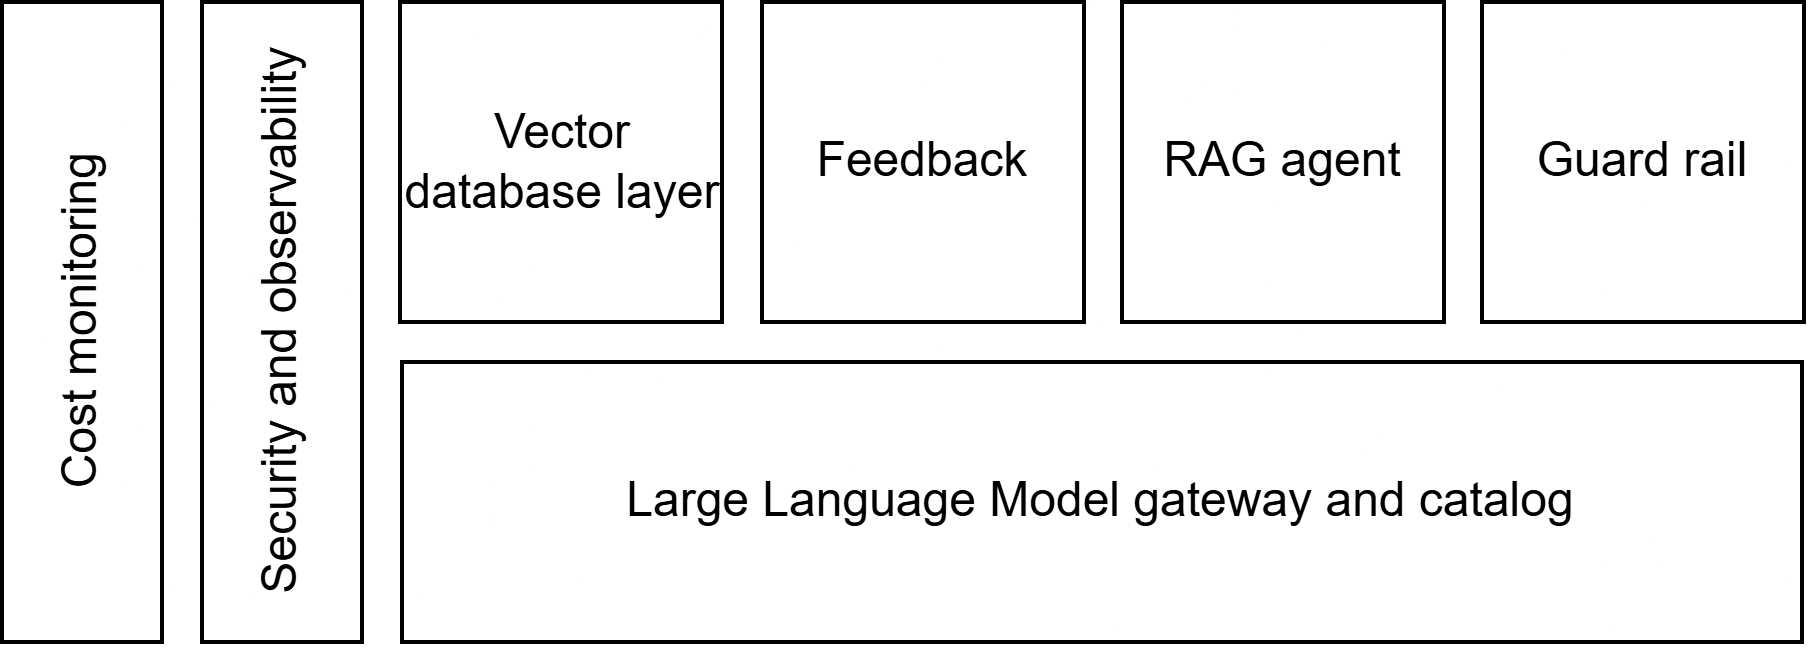
\includegraphics[width=0.5\linewidth]{images/bis14.png}
    \caption{Architecture}
\end{figure}